% SyncBox manual - Overview
% Written by Christopher Thomas.
%
% Copyright (c) 2021 by Vanderbilt University. This work is released under
% the Creative Commons Attribution-ShareAlike 4.0 International License.

\chapter{Overview}
\label{sect-over}

The {\projectname} is a device that lets a host computer and several 
instruments talk to each other. It was commissioned by the Attention 
Circuits Control Laboratory to facilitate their experiments%
\footnote{{\projectname} integration is described in:
``USE: An integrative suite for temporally-precise psychophysical
experiments in virtual environments'', Watson, M. R., Voloh, B.,
Thomas, C. J., Hasan, A. M., and Womelsdorf, T. (2018), \textit{bioRxiv},
434944  doi:10.1101/434944}.
%
A system diagram of the York University installation is shown in 
Figure \ref{fig-over-system}. A diagram of the I/O signals used by the 
{\projectname} is shown in Figure \ref{fig-over-signals}.

\begin{figure}[h]
\begin{center}
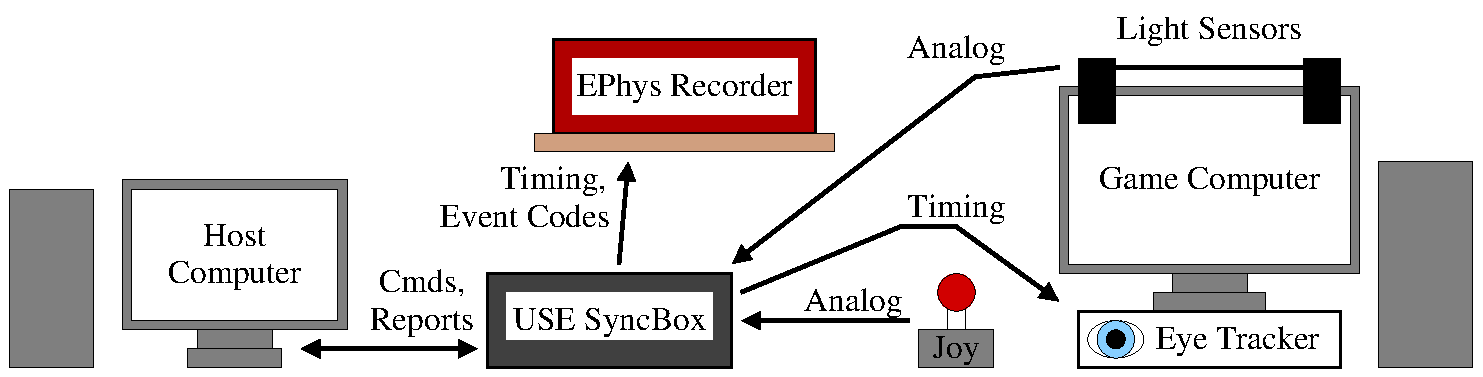
\includegraphics[width=0.9\textwidth]{figs/system.pdf}
\end{center}
\caption{System block diagram.}\label{fig-over-system}
\end{figure}

% Using the float package's "yes, _really_ here" option.
\begin{figure}[H]
\begin{center}
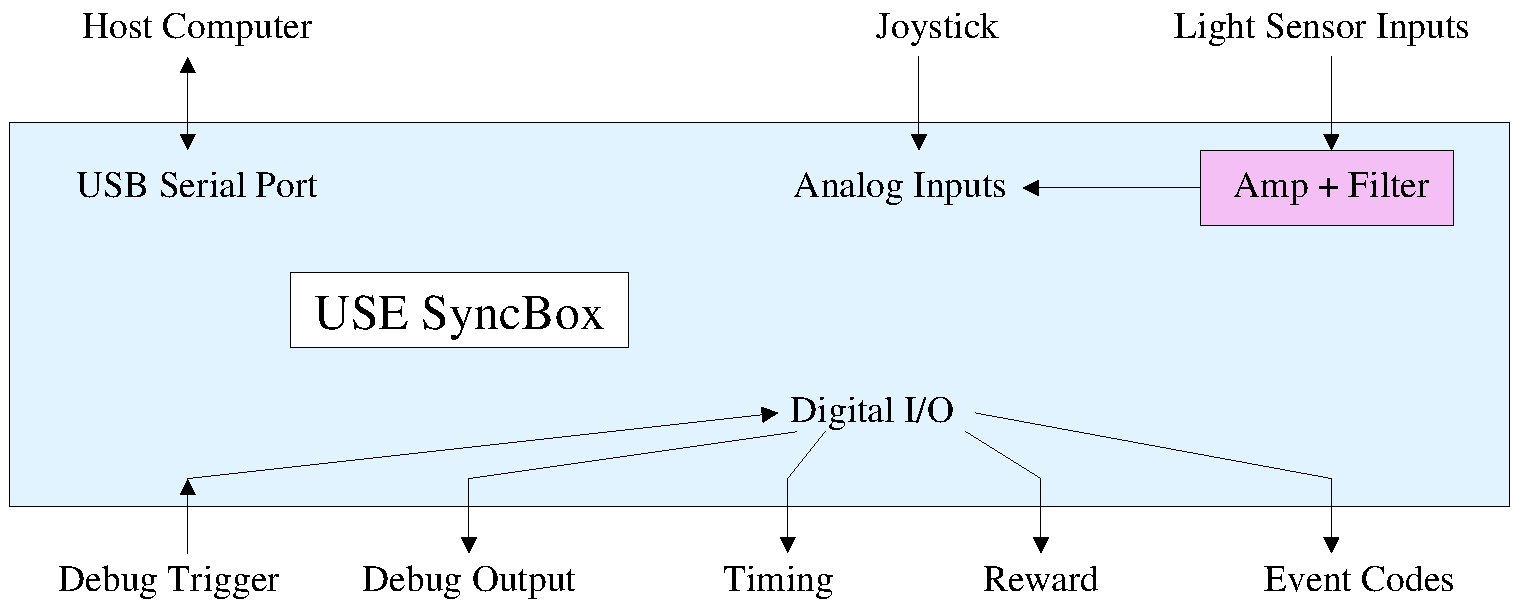
\includegraphics[width=0.8\textwidth]{figs/signals.pdf}
\end{center}
\caption{{\projectname} inputs and outputs.}\label{fig-over-signals}
\end{figure}

\clearpage
The {\projectname} handles several types of communication:

\begin{itemize}

\item It talks to the host computer over a USB serial port connection.

\item It generates timing pulses. These are controlled using the 
\textbf{Txx} series of commands. These are typically used to provide
events with known timestamps to equipment such as eye-trackers and
electrophysiology instruments.

\item It generates single pulses of variable duration. These are controlled 
using the \textbf{RWD} command. These are typically used for dispensing
a reward to test animals.

\item It emits binary number values over a parallel digital interface. 
These are controlled using the \textbf{Nxx} series of commands. These are
typically used as event codes for electrophysiology equipment.

\item It reads analog information from three general-purpose analog inputs,
and shows this data during logging. These are typically used for joystick
inputs.

\item It reads light sensors to synchronize with the game computer's 
display.  The light sensor inputs have hardware amplification and filtering
(they are special-purpose inputs, not general analog inputs).
Light levels are shown during logging.

\item Logged data is controlled using the \textbf{Lxx} series of commands.

\end{itemize}

The commands are described in detail in Section \ref{sect-commands}.

To started, connect to the {\projectname} (USB serial link at 115200 baud,
8N1), and type ``\textbf{?}'' (and enter) for help. Type ``\textbf{QRY}''
to see the {\projectname}'s settings.

The front and back panels of the {\projectname} are shown in Figure
\ref{fig-panels}. The pinout of the parallel output is shown in Figure
\ref{fig-code-pinout}.

\begin{figure}[H]
\begin{center}
\begin{tabular}{lcr}
\includegraphics[width=0.45\columnwidth]{photos/front-panel.jpg}
& ~~ &
\includegraphics[width=0.45\columnwidth]{photos/back-panel.jpg} \\
\end{tabular}
\end{center}
\caption{{\projectname} front and back panels.}\label{fig-panels}
\end{figure}

\begin{figure}[H]
\begin{center}
\includegraphics[width=0.9\columnwidth]
{pinouts/synchbox-frontpanel-pinout.png}
\end{center}
\caption{Event code connector pinout.}\label{fig-code-pinout}
\end{figure}

%
% This is the end of the file.
